\section{Results}

\begin{figure*}[!t]
  \centering
  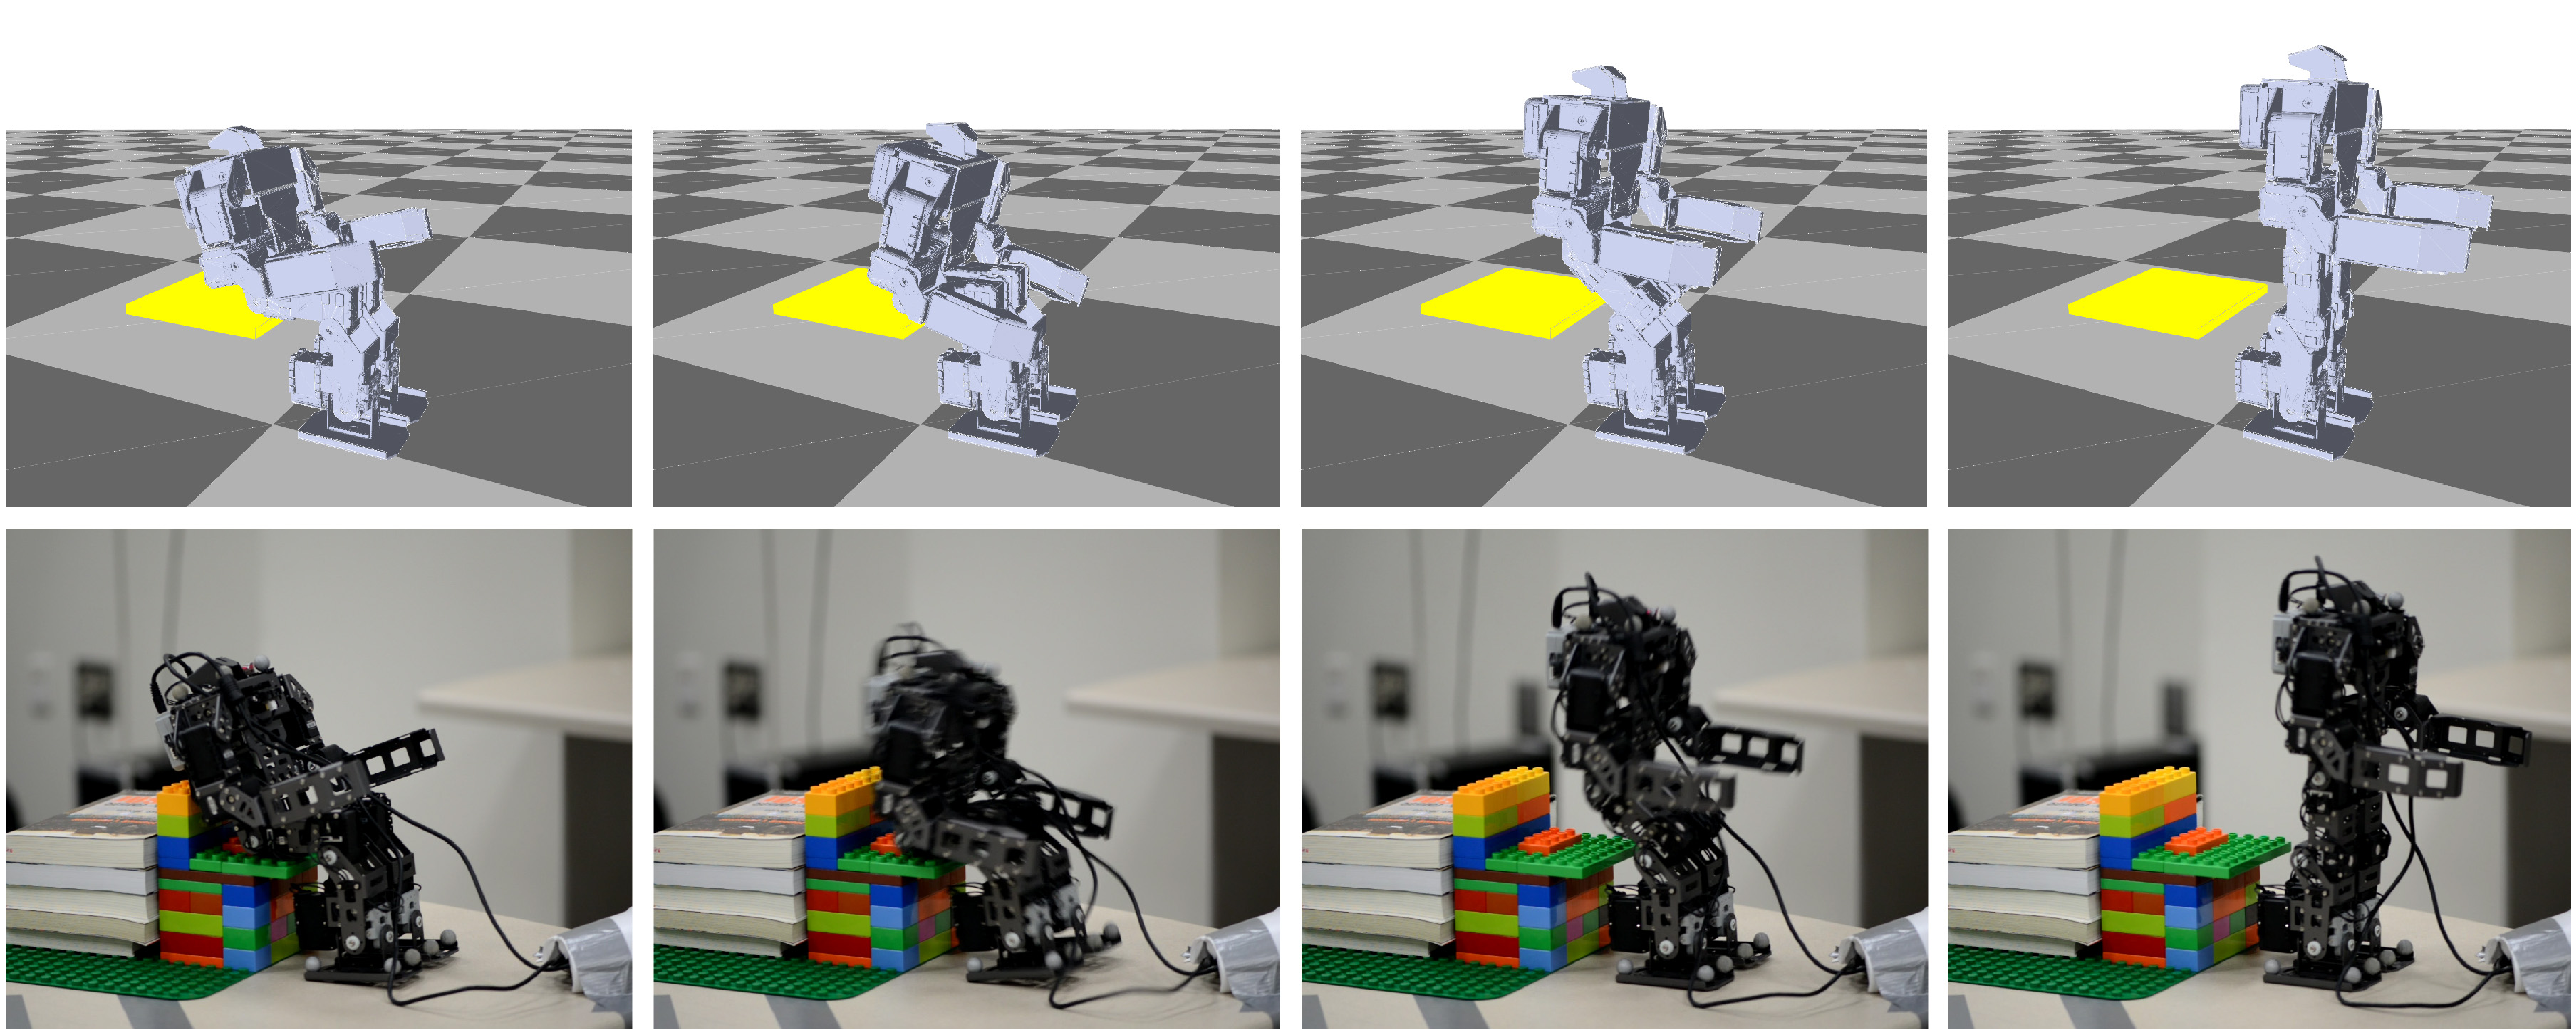
\includegraphics[width=0.95\textwidth]{figures/sit2Stand}
  \caption{The results of the sit-to-stand task in the simulation and on the real robot.}
  \vspace{-0.1in}
  \label{fig:sit2Stand}
\end{figure*}

We evaluate our system using four locomotion tasks. Please watch the accompanying video for the robot performance in the simulation and in the real world.

\subsection{Experiment Setup}

We use BIOLOID GP as our robot platform. It is a humanoid robot that consists of 18 degrees of freedom that are powered by Dynamixel AX-12/AX-18 servos. To control the robot, a master program on the PC writes the desired pose $\bar{\mathbf{q}}$ to the serial port that is connected to the robot. A slave program that runs on the robot's onboard microprocessor listens to this port and sends the desired joint angle to each actuator. At the same time, the robot performance data $\tilde{\mathbf{x}}$ is measured and sent back to the computer. We use onboard rotary encoders to measure the joint angles and a VICON motion capture system to measure the global position and orientation of the robot's torso.

Our system is implemented in C++ and runs on a laptop with a 2.6GHz quad-core CPU. We use DART to simulate the physics. We find that all the tasks can be achieved with symmetric lower body motions, which enables us to reduce the dimensionality of the control space in controller optimization. For each simulation calibration, we collect three episodes of robot data by running the same controller three times to average out the noise and other possible perturbations. Each episode is approximately two seconds. We use 32 samples per iteration and at most 50 iterations in CMA. It takes about 15 minutes to find an optimal solution in controller optimization or simulation calibration.

\begin{figure}[!b]
  \centering
  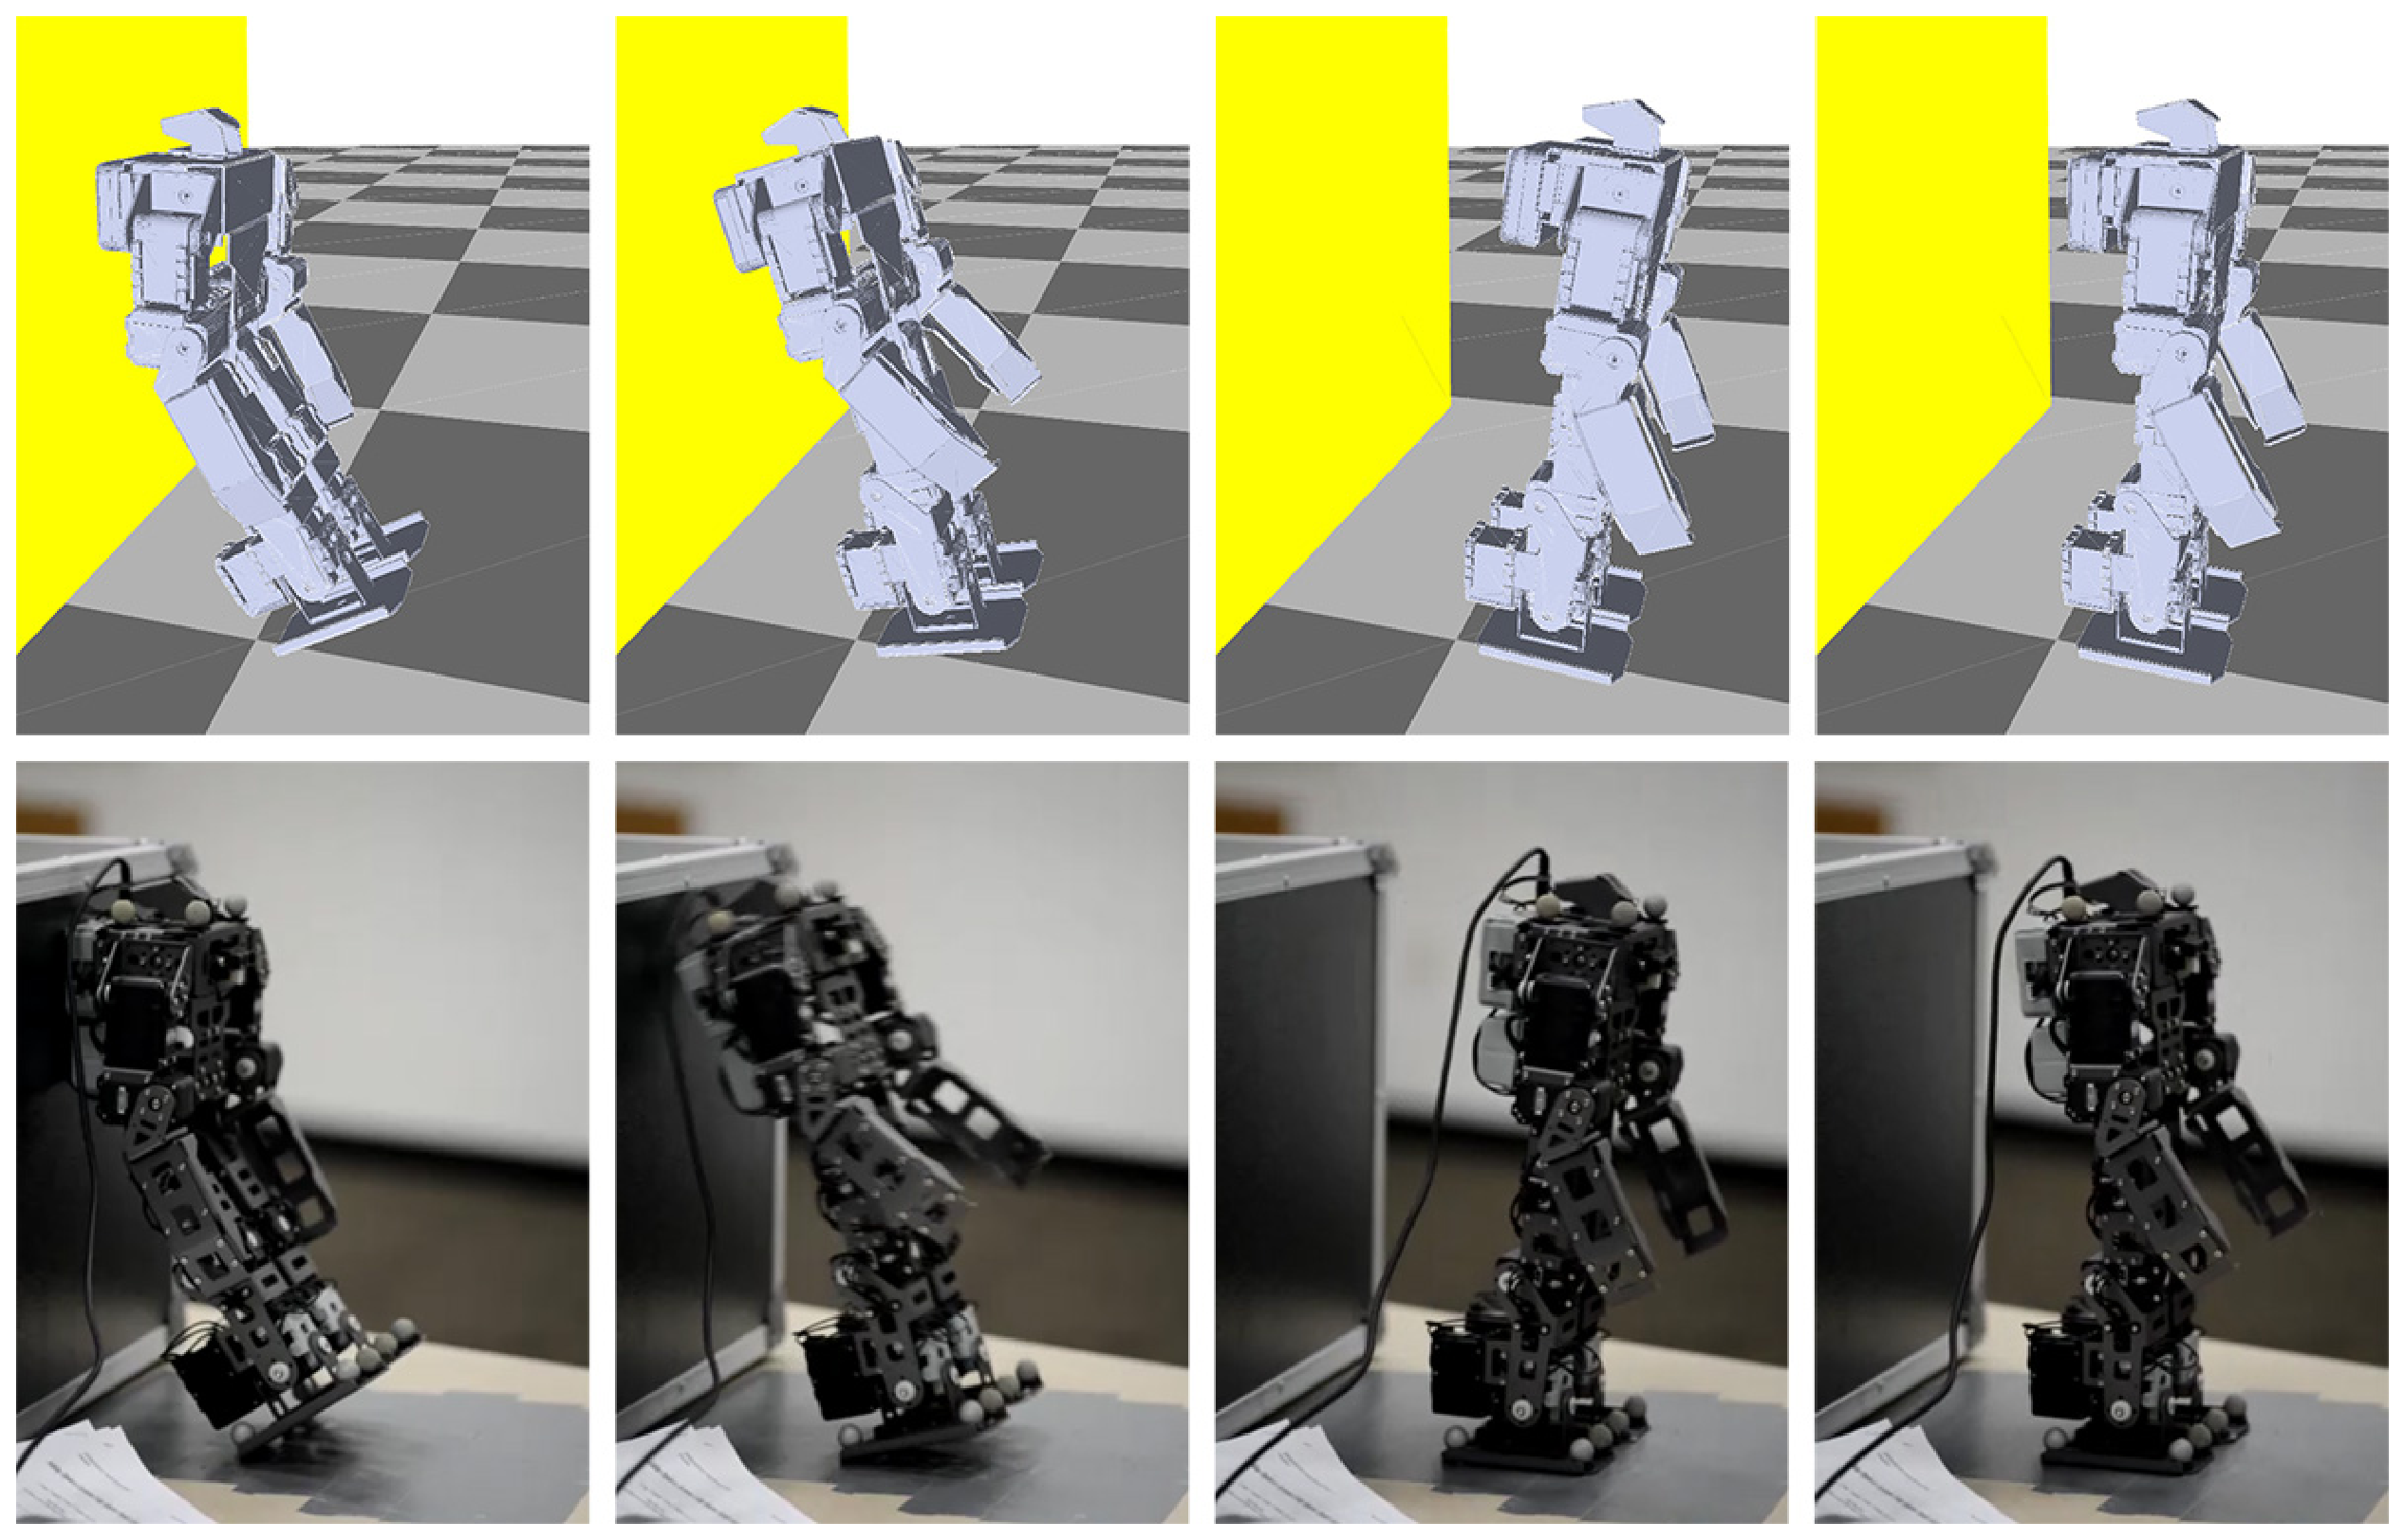
\includegraphics[width=0.45\textwidth]{figures/lean2Stand}
  \caption{The results of the lean-to-stand task in the simulation and on the real robot.}
  \vspace{-0.1in}
  \label{fig:lean2Stand}
\end{figure}

\subsection{Rising from a Sitting Position}

The first task is to rise from a chair (Figure \ref{fig:sit2Stand}). The initial and the final poses $\mathbf{q}_0$ and $\mathbf{q}_T$ are shown in the leftmost and rightmost images in Figure \ref{fig:sit2Stand}. The controller optimization needs to search for an additional inbetween keyframe $q_1$, as well as the two time intervals $t_1$ and $t_2$ between these keyframes. 

We intentionally choose the initial pose that the feet of the robot are far beyond the projection of the robot's COM in the vertical direction. If the robot simply extends the hips and the knees, it will fall backwards. This is a good test for dynamic balance. Our system successfully finds a controller that enables the robot to stand up in the simulation: the robot first accumulates a forward momentum by quickly leaning its upper body to the front. It then starts to extend the hips and the knees at the moment when the COM is moving towards the supporting feet.

When we apply this controller to the real robot, it works directly, without the need of simulation calibration. This shows that the Reality Gap is not always a problem. In some tasks, the stability region of a controller is so large that it can make the discrepancy between the virtual and the real world less critical.

\subsection{Rising from a Leaning Position}

In this task, the robot needs to rise from leaning on the wall to a standing position (Figure \ref{fig:lean2Stand}). The hip joints are initially bent and straightened out in the final configuration while all other joints do not move. The initial and the final poses are the only two keyframes for this task.

\begin{figure}[!b]
  \centering
  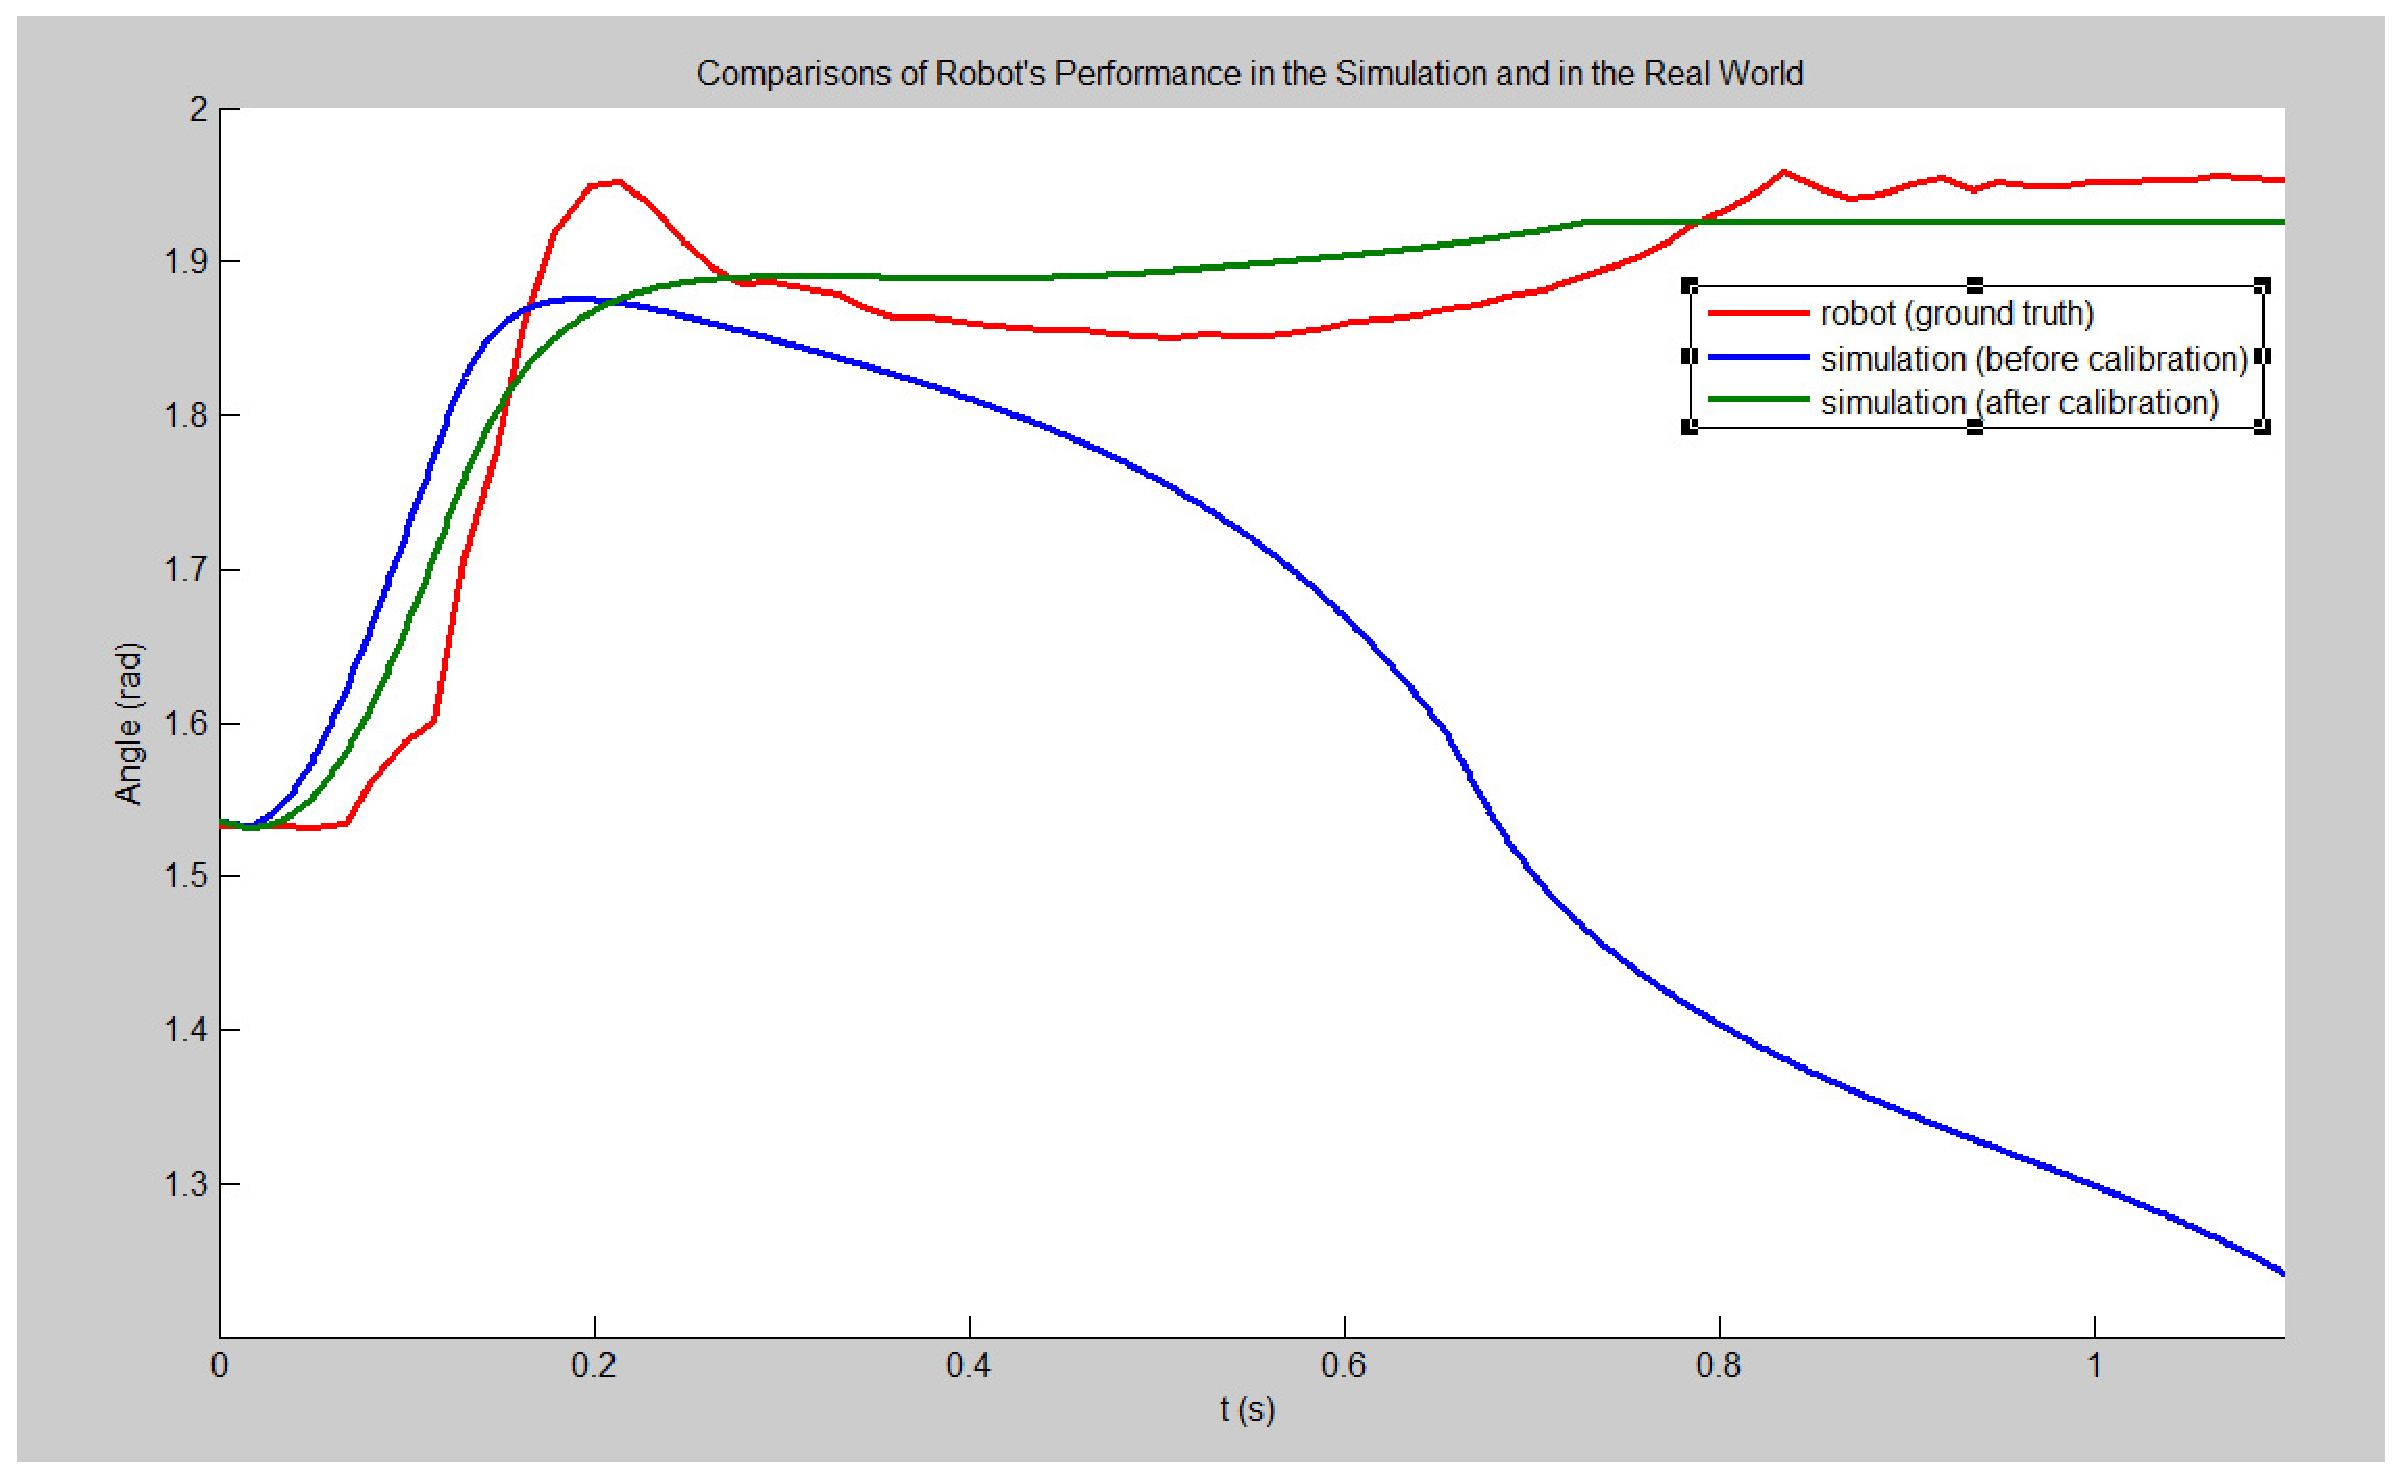
\includegraphics[width=0.3\textwidth]{figures/simRobotCompare}
  \caption{Comparisons of the robot's global orientation over time in the simulation (before/after calibration) and in the real environment.}
  \vspace{-0.1in}
  \label{fig:simRobotCompare}
\end{figure}


\begin{figure*}[!t]
  \centering
  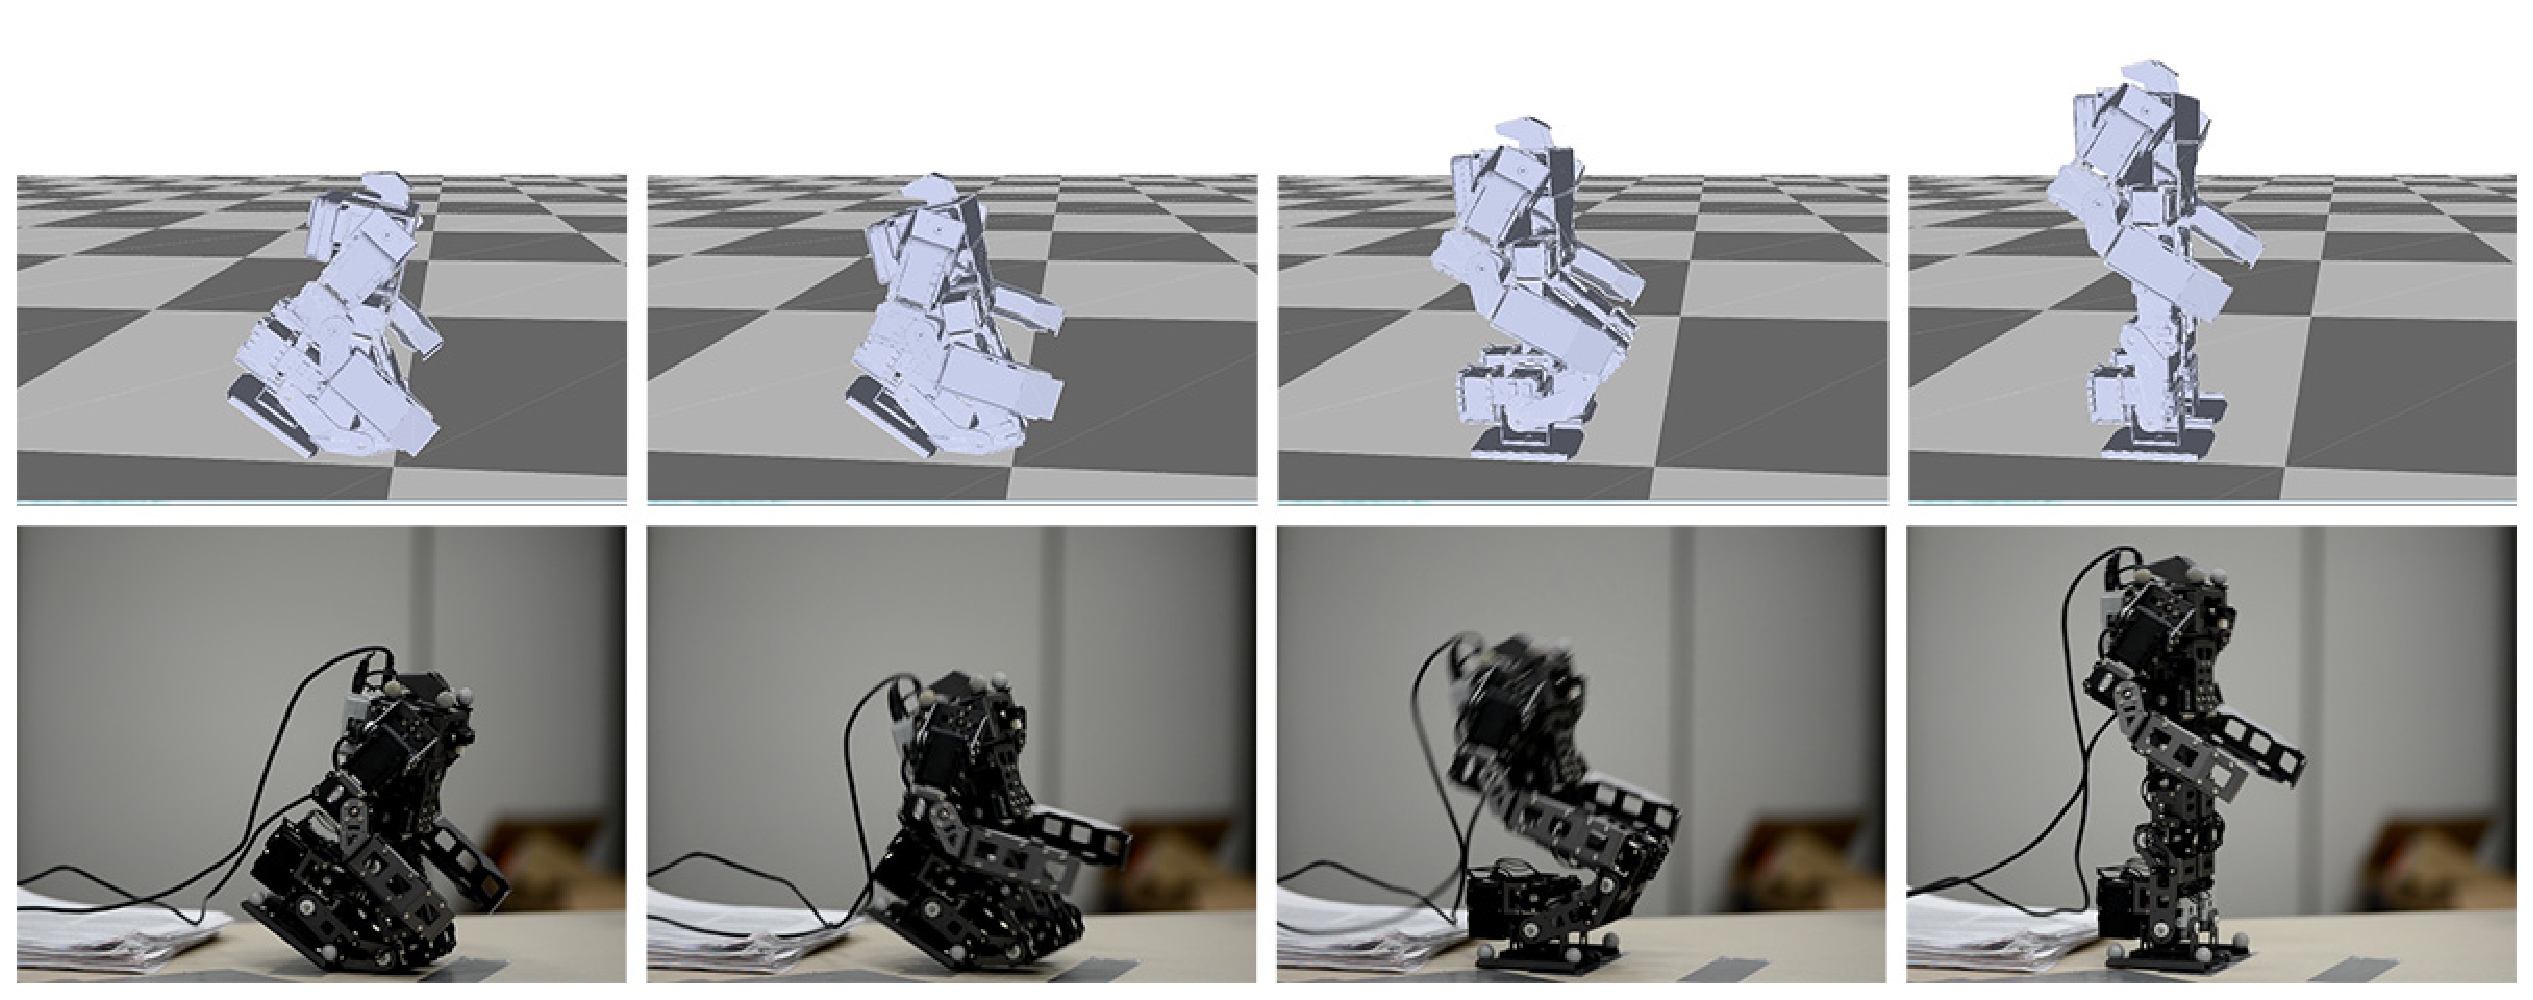
\includegraphics[width=0.95\textwidth]{figures/kneel2Stand}
  \caption{The results of the kneel-to-stand task in the simulation and on the real robot.}
  \vspace{-0.1in}
  \label{fig:kneel2Stand}
\end{figure*}

\begin{figure*}[!t]
  \centering
  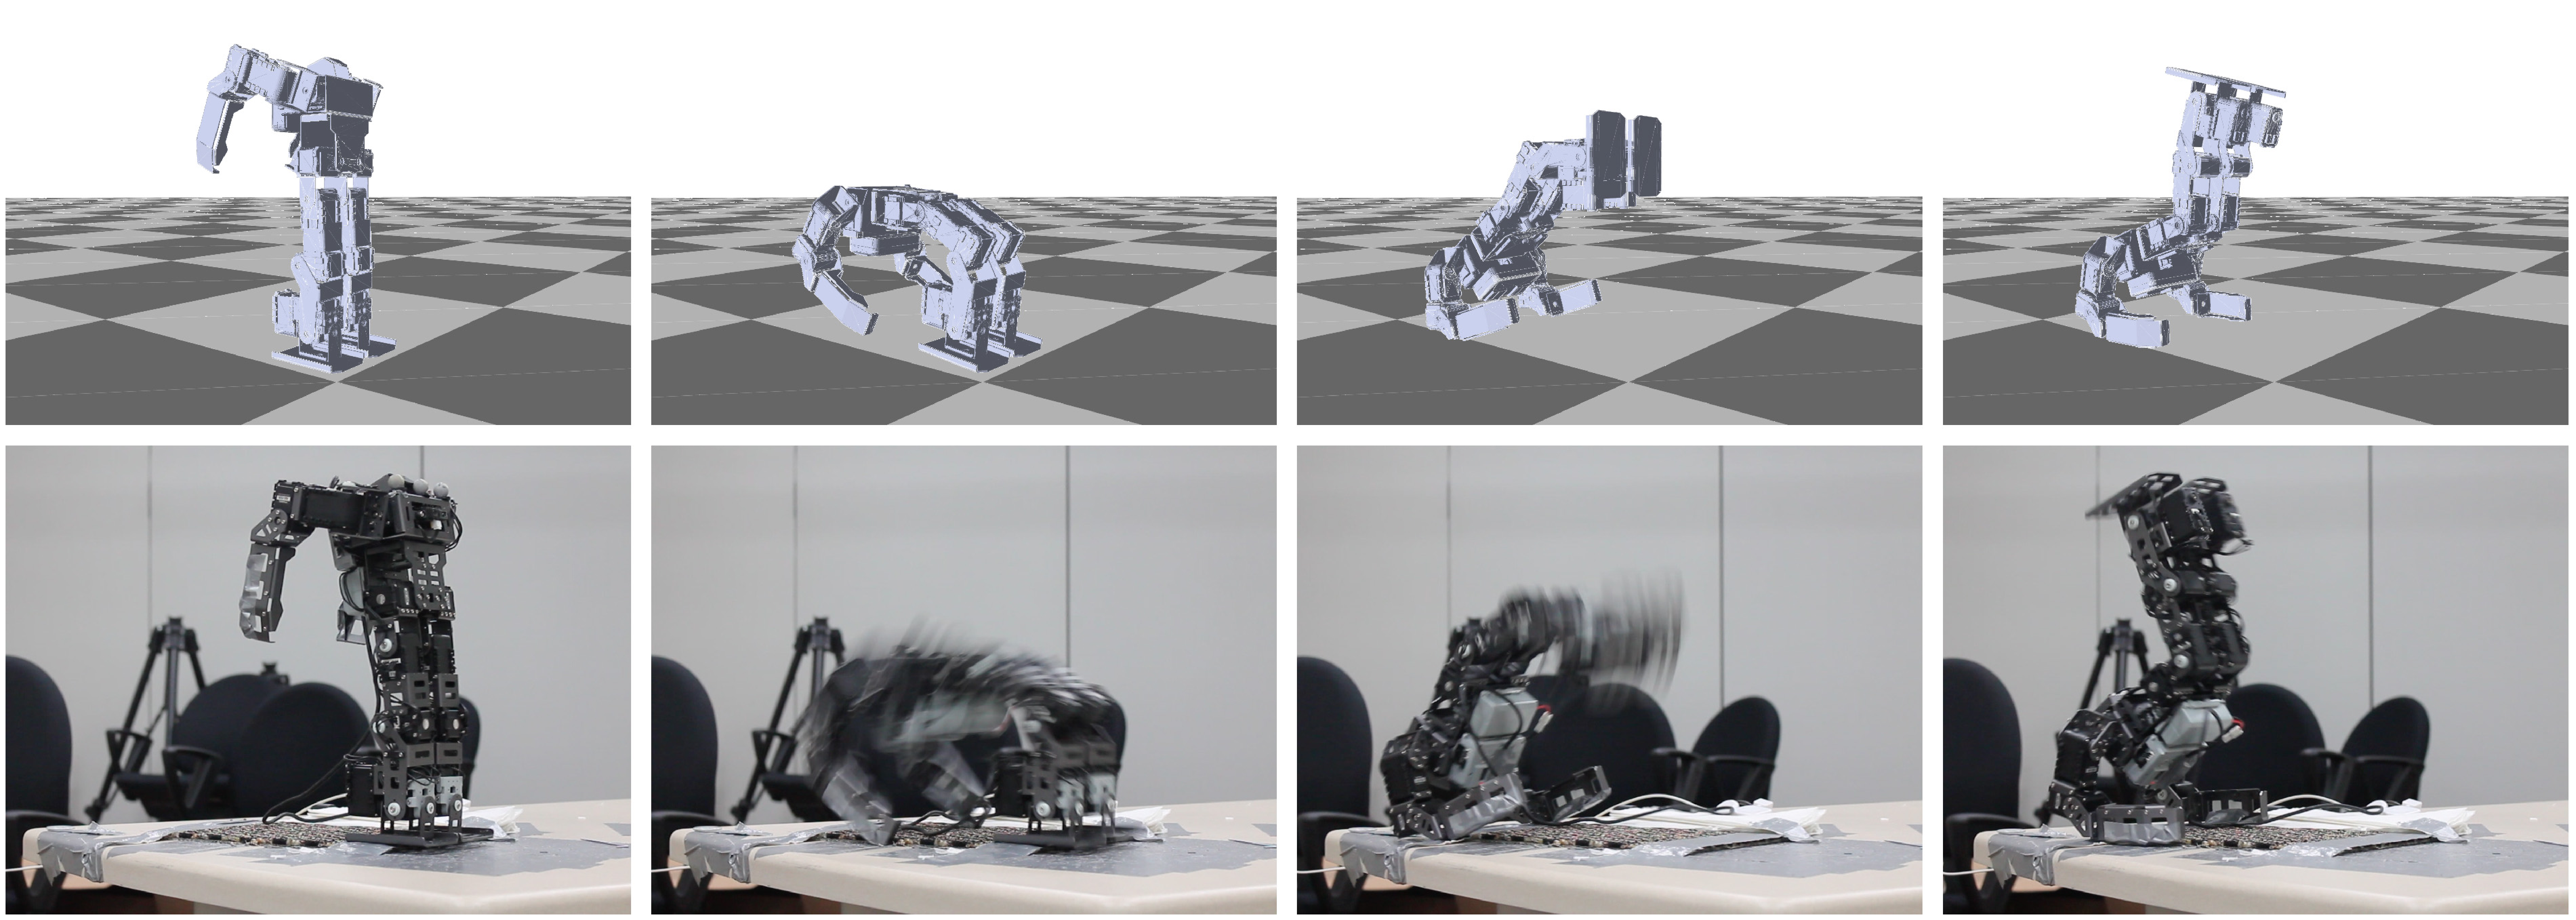
\includegraphics[width=0.95\textwidth]{figures/stand2Hand}
  \caption{The results of the stand-to-handstand task in the simulation and on the real robot.}
  \vspace{-0.1in}
  \label{fig:stand2Hand}
\end{figure*}

The goal of controller optimization is to find an appropriate time interval $T$ between these two keyframes. If the time interval is too long, the robot cannot accumulate enough momentum to rise. If this time interval is too short, the robot can bounce off the wall too quickly and fall forward. Without simulation calibration, the controller optimization cannot find a successful controller for this task: The robot cannot rise when $T > 0.11s$ and overshoots when $T \leq 0.11s$. Nevertheless, we apply the controller with the highest fitness value $T=0.11s$ on the robot. In contrast to the simulation result, in which the simulated robot rises too quickly and falls forward, the robot in the real world actually cannot rise. Figure \ref{fig:simRobotCompare} compares the trajectories of the robot's global orientation in the simulation (blue curve) and in the real world (red curve). After one iteration of simulation calibration, the discrepancy is greatly reduced (Figure \ref{fig:simRobotCompare} green curve). We optimize the controller again in this calibrated simulator. This time, the optimal controller works both in the simulated and in the real world. We successfully cross the Reality Gap with one iteration of simulation calibration, which only needs about 6 seconds of robot data.



\ignorethis{
\begin{figure}[!b]
  \centering
  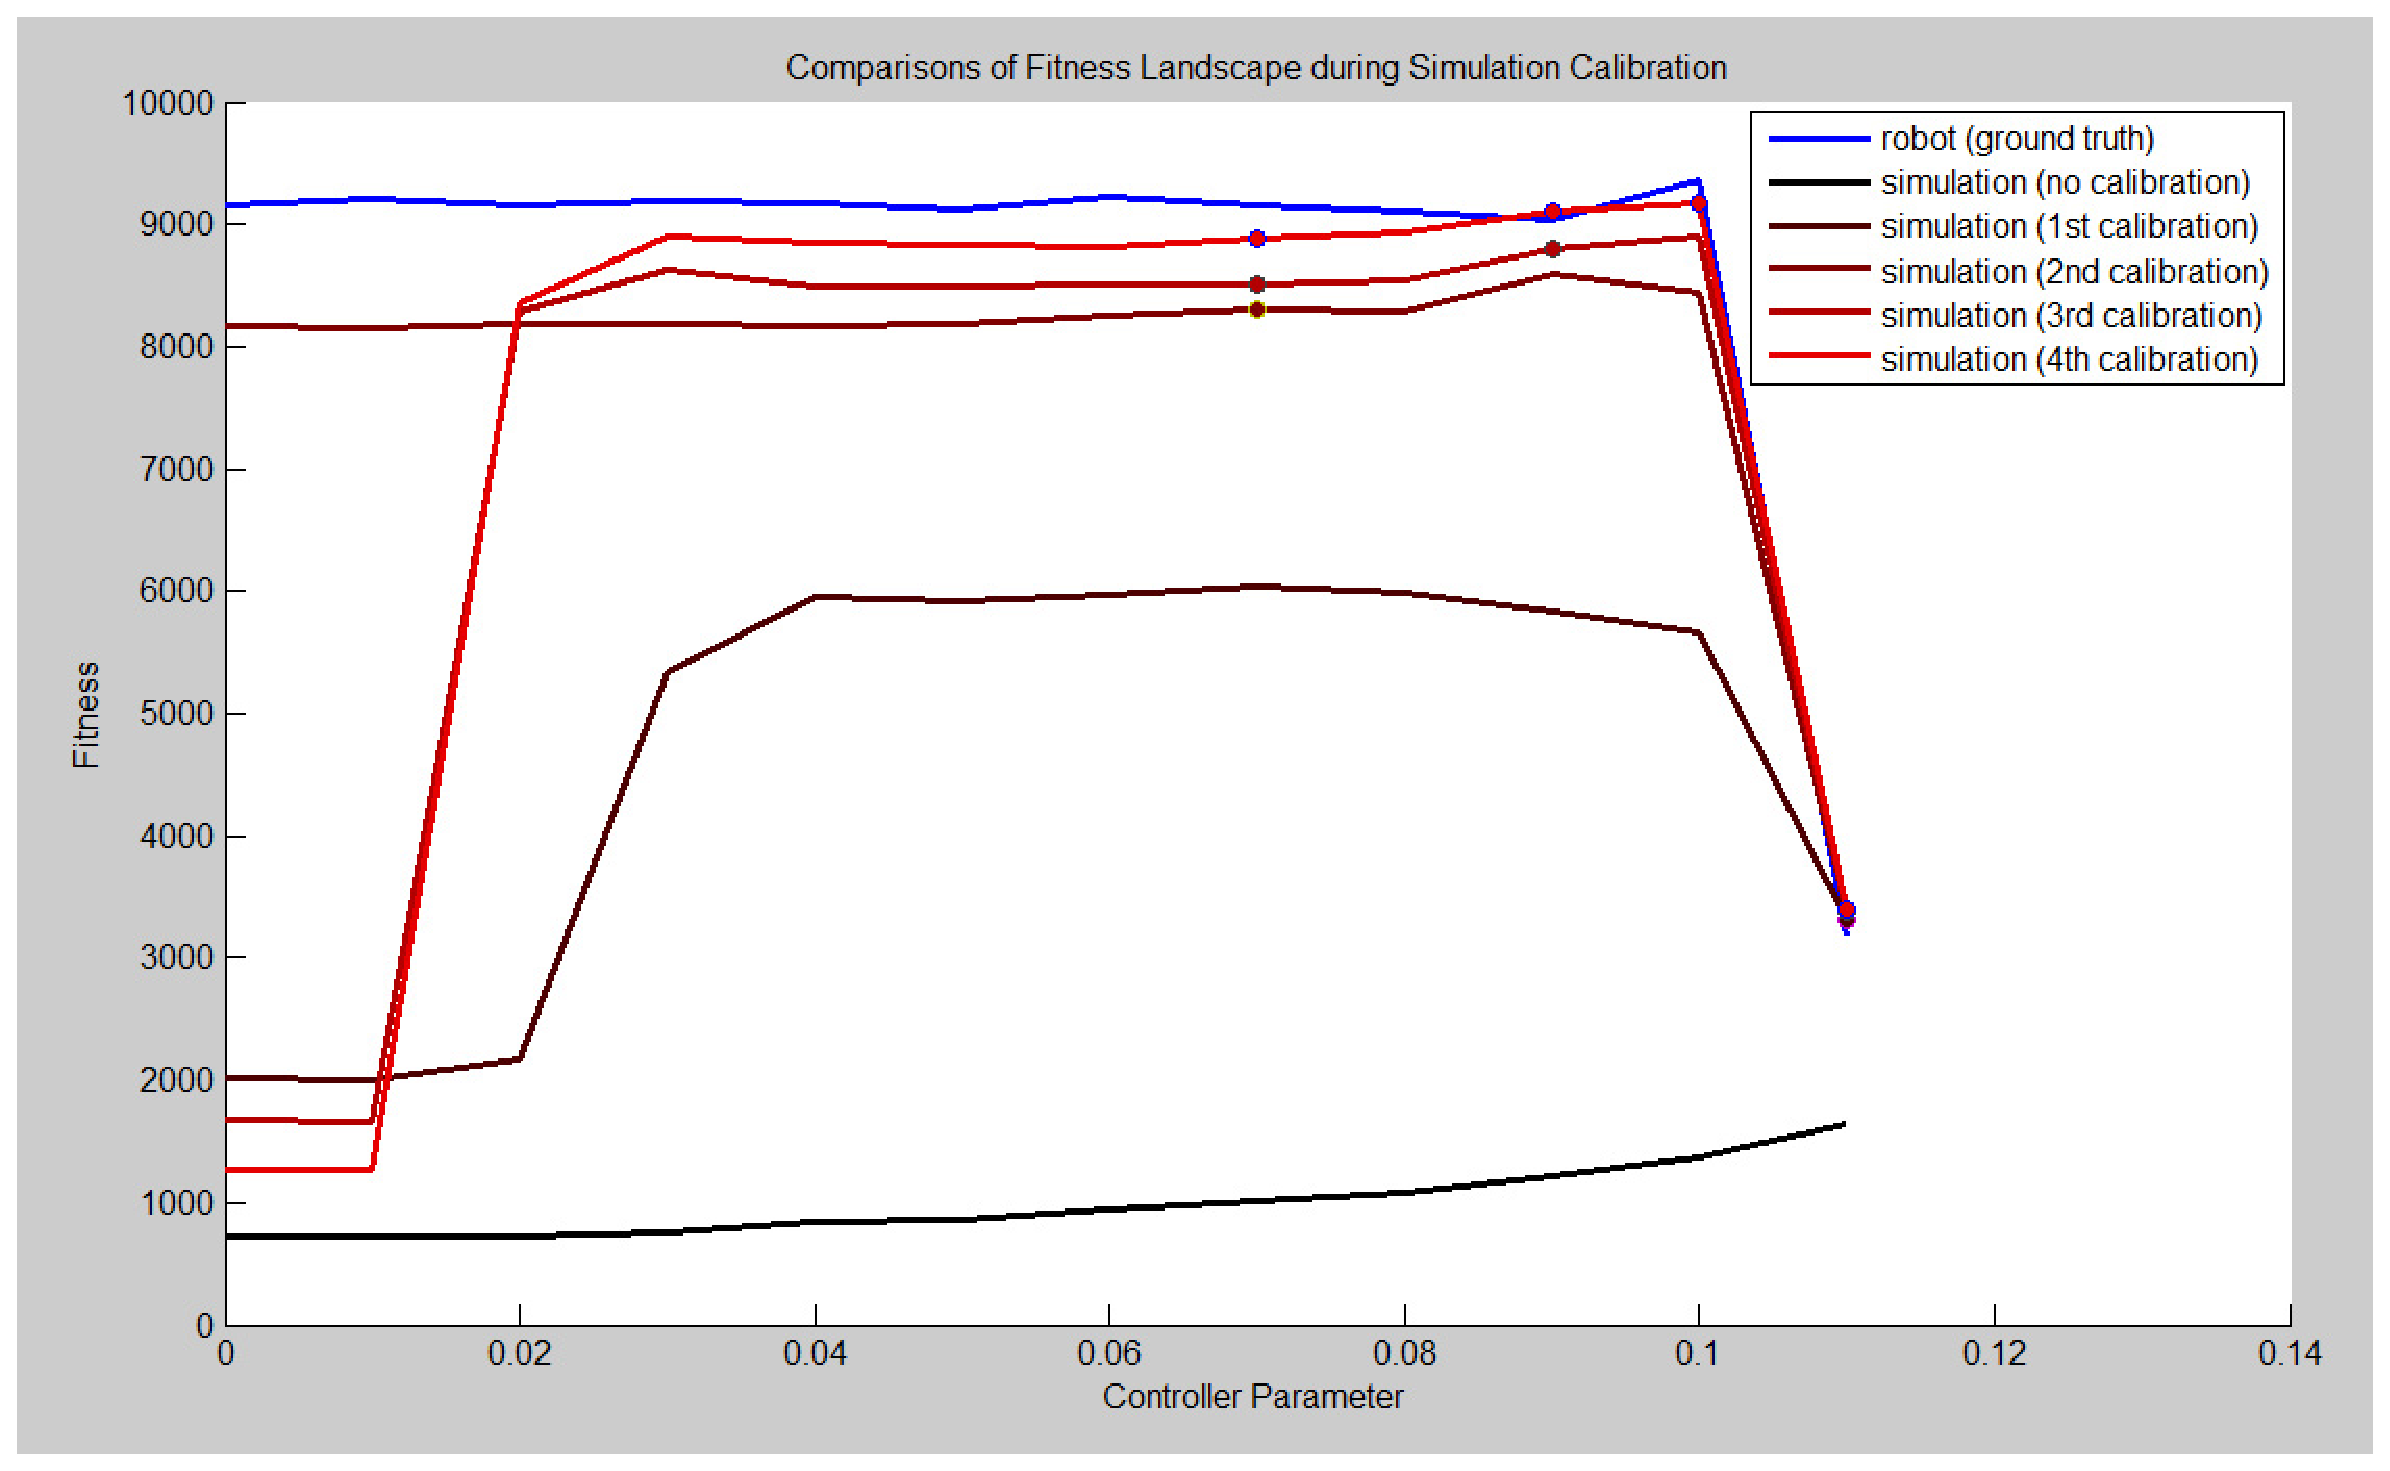
\includegraphics[width=0.4\textwidth]{figures/fitnessLandscape}
  \vspace{-0.1in}
  \caption{Comparisons of the fitness landscape as more iterations of simulation calibration are performed.}
  \label{fig:fitnessLandscape}
\end{figure}


To better understand how the Reality Gap is gradually narrowed by simulation calibration over multiple iterations, we perform an additional evaluation. Figure \ref{fig:fitnessLandscape} shows how the fitness landscape in the simulation changes with different number of iterations of simulation calibration. The blue curve is the ground truth. It is evaluated on the real robot by varying the control parameter $T$ in the range of $[0, 0.11]$. The fitness value is calculated according to eq. (\ref{eqn:controllerObj}). The fitness landscape stays at a high value when $T\in[0, 0.1]$, which means that the real robot can successfully rise if the controller uses less than 0.1s to change the pose from the initial to the final configuration. In contrast, without simulation calibration, the fitness landscape (lowest black curve) stays at a low value for the entire control space. In other words, no controller exists that can make the robot stand up in the simulation. The gap between the blue and the black curves is analogue to the Reality Gap. One iteration of simulation calibration brings the fitness landscape in the simulation towards the ground truth. As more iterations are performed, the fitness landscape in the simulation (brown and red curves) gradually approaches the ground truth, and the Reality Gap is narrowed in this process. Note that a large discrepancy still exists in the region of the parameter space where $T<0.02s$. This is probably caused by two reasons. First, in the region of $T<0.02s$, the torque output of the servo is at its limit but the torque limit is not considered in simulation calibration. Second, the controllers and the data (the red circles in Figure \ref{fig:fitnessLandscape}) that we use in simulation calibration concentrate on the right half of the parameter space, which makes it difficult to generalize to a region where the data is scarce ($T<0.02$). However, this is beneficial in our applications because the computational resource is focused at the important regions near the successful controllers. This explains why our system can find a successful controller in the real word with minimal robot experiments.
}

\subsection{Rising from a Kneeling Position}

Figure \ref{fig:kneel2Stand} shows that the robot stands up from a kneeling pose. Between the user-specified initial and final poses, the optimal controller consists of two additional keyframes. It demonstrates an agile getting-up motion in the simulation: The robot first leans its upper-body backwards. As its COM is moving to the back, it quickly bends the hip, flexes its ankles and stands up. This entire motion resembles one of the most agile ways that we human get up from a kneeling position when we do not use our hands for additional support. Although this controller works perfectly in the simulation, the robot falls backward in the real world. After simulation calibration, we optimize a new controller, with which the robot can successfully stand up from in the real world.

\subsection{Flipping to a Handstand Position}
We test our system with a challenging gymnastic action: flipping to a handstand position from a standing pose (Figure~\ref{fig:stand2Hand}). There are two unique challenges in this task. First, the speed and the curvature of the initial arching motion is crucial and only a narrow range of such speed and curvature can lead to a balanced handstand. Second, the USB cable that connects the robot to the computer will inevitably hit the ground during the backflip, which injects a strong perturbation that is not modeled in our simulation.

With two iterations of simulation calibration and controller optimization, our system finds a successful controller that works both in the simulation and in the real world: The robot arches back rapidly and lifts its feet after the arms touch the ground. It shows that our system can automatically design controllers for challenging locomotion tasks, even with strong unmodeled perturbations.

